\section{Method}\label{sec:method}
This section describes LightGCN, NGCF and PUP.
The difference between these recommendation models are described with focus on the adjacency matrix and the embeddings.
We describe the implementation for our hypothesis in the following section.
Our hypothesis is: Changing the input parameters to include price and categories for LightGCN and NGCF will model price-aware recommendation through convolutions and thereby achieve more precise recommendation.
% An attempt at implementing price aware recommendation in LightGCN and NGCF is described, where the focus is on changing the input parameters.
\subsection{LightGCN and NGCF}\label{subsec:lightgcn-ngcf}
In LightGCN Xiangnan et al. investigate the effect of feature transformation and nonlinear activation functions within collaborative filtering using NGCF \cite{lightgcn}.
NGCF is a framework developed by Wang et al. \cite{NGCF_2019} that utilizes a Graph Neural Network with three components in the framework: (1) an embedding layer that constructs initial user - and item embeddings; (2) embedding propagation layers that capture CF with the two operations of message construction and message aggregation; (3) a prediction layer that concatenates the embeddings at each layer for each user and for each item such that $e_{u}^{(*)} = e_{u}^{(0)}||...||e_{u}^{(l)}$ and $e_{i}^{(*)} = e_{i}^{(0)}||...||e_{i}^{(l)}$ where $u$ indicates the user, $i$ indicates the item, $e$ is the embedding and $l$ is the layer \cite{NGCF_2019}.
Within the second component of message construction the message embedding is implemented as:
\begin{equation}
    m_{u \leftarrow i} = \frac{1}{\sqrt{|\mathcal{N}_u||\mathcal{N}_i|}}(W_1e_i + W_2(e_i \odot e_u)),
    \label{eq:message-construction}
\end{equation}
where $W_1$ and $W_2 \in R^{d' \times d}$ are weight matrices, $d$ is the embedding size and $d'$ is the transformation size.
$\frac{1}{\sqrt{|\mathcal{N}_u||\mathcal{N}_i|}}$ is the graph Laplacian norm, where $\mathcal{N}_u$ and $\mathcal{N}_i$ are the set of neighbors of user $u$ and item $i$.
This is done with the purpose of calculating how much the item contributes to the users preference \cite{NGCF_2019}.
LightGCN criticize the use of feature transformation in the form of weight matrices $W_1$ and $W_2$ as not being useful for CF as each user-item interaction graph only has the ID as input and it has no semantic value \cite{lightgcn}.
Also within the second component the message aggregation is implemented as:
\begin{equation}
    e_{u}^{(l)} = \mbox{LeakyReLU}(m^{(l)}_{u \leftarrow u} + \sum^{}_{i \in \mathcal{N}} m^{(l)}_{u \leftarrow i}),
\end{equation}
where $e_{u}^{(l)}$ is the embedding of user $u$ at layer $l$.
LeakyReLU is the nonlinear activation function used in NGCF to allow encoding positive and small negative signals.
LightGCN shows that NGCF will perform better if the feature transformation is removed, and that the activation function has a small effect when feature transformation is included, but if feature transformation is disabled the activation function will have a negative impact on performance.
LightGCN also shows that NGCF will significantly improve if both the activation function and feature transformation are removed \cite{lightgcn}.

\subsection{Price-aware Recommendation with Graph Convolutional Networks}\label{subsec:PUP}
Yu Zheng et al. develops an effective method called \textit{Price-aware User Preference-modeling (PUP)} that is used to create recommendations with focus on the price factor \cite{Priceaware}.
There are two main challenges.
The first is that the preferences of a user on item price are unknown, and can only be seen implicitly by previous purchases.
The second challenge is that the price of an item largely depends on what category the item is within.
For the first problem they propose a model that creates a relationship between user-to-item and item-to-price using a Graph Convolutional Network, so that they can propagate the influence of price onto the users.
For the second problem they solve this by integrating the categories and items into the propagation process.
PUP represents the data as a heterogeneous undirected graph $G = (V,E)$ where the nodes in $V$ consist of user nodes $u \in U$, item nodes $i \in I$, category nodes $c \in \textbf{c}$, and price nodes $p \in \textbf{p}$.
The edges in $E$ consist of interaction edges $(u, i)$ with $R_{ui} = 1$ if there is an interaction between user $u$ and item $i$ and category edges $(i, \textbf{c}_i)$ and price edges $(i, \textbf{p}_i)$.
Traditional Latent Factor Models such as Matrix Factorization only take a single type of edge $(u, i)$ into account.
This makes them insufficient when multiple types such as $(u, p)$ and $(i, c)$ are introduced \cite{Priceaware}.
Hereby Yu Zheng et al. use a Graph Neural Network to learn the embeddings so that each node has a separate embedding $e' \in \mathbb{R}^d$ where d is the dimensions of the embeddings.
In GCN the nodes propagate its nearest neighbors, which could be user-item, item-price or item-category.
Embeddings from node j to node i are propagated as follows:
\begin{equation}
    t_{ji} = \frac{1}{|\mathcal{N}_i|}e'_j,
\end{equation}
where $\mathcal{N}_i$ is the set of neighbors for node $i$ and $e'_j$ is the embedding node j.
The updating rule is:
\begin{align*}
     & o_u = \sum_{j \in \{i \textrm{ with } R_{ui}=1 \} \cup \{ u\}}^{} t_{ju}                            \\
     & o_i = \sum_{j \in \{u \textrm{ with } R_{ui}=1 \} \cup \{ i, \textbf{c}_i \textbf{p}_i\}}^{} t_{ji} \\
     & o_c = \sum_{j \in \{i \textrm{ with } \textbf{c}_i=c \} \cup \{ c\}}^{} t_{jc}                      \\
     & o_p = \sum_{j \in \{i \textrm{ with } \textbf{p}_i=c \} \cup \{ p\}}^{} t_{jp}                      \\
     & e_f = \textrm{tanh}(o_f), f \in \{u, i, c, p\},
\end{align*}
where $e_u$, $e_i$, $e_c$, and $e_p$ are the embeddings for user $u$, item $i$, category $c$ and price $p$.
The intuition about this updating rule is that the node gets aggregated together with its neighbors and in each layer it will go one step further.
So for example a price nodes embedding will be aggregated together with all item node embeddings connected with this specific price.
By doing this items with the same price levels are expected to be more similar than items not in the same price level.
The intuition about the category is the same as with the price.
The final purchase prediction $s$ between user $u$ and item $i$ is formulated as follows:
\begin{equation}
    s = e^T_u e_i + e^T_u e_p + e^T_i e_p + \alpha (e^T_u e_c + e^T_u e_p + e^T_c e_p),
\end{equation}
where $\alpha$ is a hyper-parameter used to balance the categories influence on the prediction.
The results of a Top-K Recommendation Performance test showcase that PUP outperforms other state-of-the-art methods such as NGCF with an average improvement of 3.59 \% to 5.97 \% \cite{Priceaware}.

\subsection{Generated adjacency matrix}
In the following subsection the generated adjacency matrices of LightGCN and price aware recommendation are described.
Both use the adjacency matrix as a representation for a heterogeneous graph, where the value 1 represent a connection between two nodes.

\subsection{LightGCN}
For LightGCN the adjacency matrix is the size of $\textrm{number of users} + \textrm{number of items} \times \textrm{number of users} + \textrm{number of items}$.
Then for every connection between item $i$ and user $u$ 1 is inserted.
It is generated with SciPy that creates a dictionary of keys, where two keys indicate the position in the matrix, and the value is 1 if there is a connection. 
As users are unable to have a connection with other users, and the same with items, they are able to exploit this by inserting all connections from users to items, and then transposing the matrix.

\subsection{Price-aware recommendation}
The adjacency matrix in price-aware recommendation is also implemented as a sparse matrix using SciPy.
This is done by creating two arrays, row and column.
The row and column are both the length of all interactions plus two times the amount of items.
We start by for each user inserting their id as many times to the array as the number of items that they have interacted with.
The id's of the items that the user interacted with are mapped to the corresponding index in the column array.
After all user item interactions have been mapped to the row and column arrays, the item prices and category relationships are mapped to the arrays.
This is done by inserting the index of an item into the row twice.
At the indexes where the item was added to the row, the corresponding category and price related to that item are inserted to the column.
A third array is created with the length of row where ones are inserted.
Using this array, column and row can create a sparse adjacency matrix by mapping the index $i$ in row and column to the array with ones.
Within the adjacency matrix, there will be inserted 1 if there is a connection between item $i$ and user $u$, item $i$ and category $c$, and item $i$ and price $p$.
This results in a adjacency matrix that is of size number of users + number of items + number of categories + number of prices $\times$ number of users + number of items + number of categories + number of prices.

\subsection{Embeddings comparison}
In the following subsections the embeddings of LightGCN, NGCF and Price-aware recommendation are described.
Unlike with the adjacency matrices, the difference between the embeddings of NGCF and LightGCN are significant here.
For all nodes including categories and prices, the only value used is the node ID.
They utilize the embedding layer to compress the one-hot ID encoding to embeddings, so that each node has a separate embedding $e' \in \mathbb{R}^d$, where $d$ is the dimension size.

\subsubsection{LightGCN}\label{subsubsec:lightgcn-embedding}
The embeddings for LightGCN are constructed as follows \cite{lightgcn},
\begin{equation}
    E^{(k+1)} = (D^{\frac{1}{2}}AD^{\frac{1}{2}}E^{(k)}),
\end{equation}
where $A$ is the adjacency matrix containing users and items (described in \autoref{subsubsec:lightGCN-adj}) and $D$ is a diagonal matrix, where $D_{ii}$ denotes the sum of the $i-th$ row in the adjacency matrix $A$.
The $0th$ layer embedding is initialized as random normalized values, where $E^{(0)} \in R^{(I + U)\times T}$, and $T$ is the embedding size.
The final embedding is obtained as follows,

\begin{equation}
    e_u = \sum_{k=0}^{K} \alpha_k e_u^{(k)};\;\;\; e_i = \sum_{k=0}^{K} \alpha_k e_i^{(k)},
\end{equation}
where $\alpha$ is set to $1/(K + 1)$ and is used to normalize the embeddings.
$K$ is the number of layers defined, and $k$ is the current layer.

\subsubsection{NGCF}\label{subsubsec:NGCF-embed}
The embeddings for NGCF are constructed as follows \cite{NGCF_2019},
\begin{equation}
    \begin{split}
        E^{(l)} = &LeakyReLU((\lambda + I)E^{(l-1)}W_1^{(l)}+\\
        & \lambda E^{(l-1)}\bigodot E^{(l-1)}W_2^{(l))},
    \end{split}
\end{equation}
where $E^{(l)} \in \mathbb{R}^{I+U \times T}$ are the item and user embeddings after $l$ convolutions.
$E^{(0)} \in \mathbb{R}^{I+U \times T}$ is the $0th$ layer embedding, where $T$ is the embedding size.
$I$ is the identity matrix.
$W_1^{(l)}$ and $W_2^{(l)}$ are trainable weight matrices.
$\lambda$ is the Laplacian matrix for the user-item, item-price and item-category graph, and is defined as follows:
\begin{equation}
    \lambda = D^{\frac{1}{2}}AD^{\frac{1}{2}},
\end{equation}
where $A$ and $D$ are the adjacency and diagonal matrix.

\subsubsection{Price-aware recommendation}\label{subsubsec:price}
The input parameters when constructing the embeddings are the adjacency matrix $A \in \mathbb{R}^{N \times N}$ and identity matrix $I \in \mathbb{R}^{N \times N}$, where $N$ is the number of nodes.
Embeddings from node j to node i are propagated as follows \cite{Priceaware},
\begin{equation}
    t_{ji} = \frac{1}{|\mathcal{N}_i|}e'_j,
\end{equation}
where $\mathcal{N}_i$ is the set of neighbors for node $i$ and $e'_j$ is the embedding node j.
The updating rule is,
\begin{equation}
    \begin{split}
        & o_u = \sum_{j \in \{i \textrm{ with } R_{ui}=1 \} \cup \{ u\}}^{} t_{ju}                            \\
        & o_i = \sum_{j \in \{u \textrm{ with } R_{ui}=1 \} \cup \{ i, \textbf{c}_i \textbf{p}_i\}}^{} t_{ji} \\
        & o_c = \sum_{j \in \{i \textrm{ with } \textbf{c}_i=c \} \cup \{ c\}}^{} t_{jc}                      \\
        & o_p = \sum_{j \in \{i \textrm{ with } \textbf{p}_i=c \} \cup \{ p\}}^{} t_{jp}                      \\
        & e_f = \textrm{tanh}(o_f), f \in \{u, i, c, p\},
    \end{split}
\end{equation}
where $e_u$, $e_i$, $e_c$, and $e_p$ are the embeddings for user $u$, item $i$, category $c$ and price $p$ respectively.
These embeddings are used to compute the predictions as described in \autoref{subsec:price-intro}.

\subsubsection{Differences in embeddings}
The difference between NGCF and LightGCN are that NGCF utilizes the $LeakyReLU$ activation function as well as using the trainable weight matrices.
While NGCF and LightGCN are constructed for collaborative filtering without additional side information, the construction of the embeddings in Price-Aware recommendation focuses on constructing additional embeddings for both price and category, and utilizing these to compute predictions.

\subsection{Simple price aware extension of LightGCN}\label{subsec:simple-extension}
\begin{figure}
    \centering
    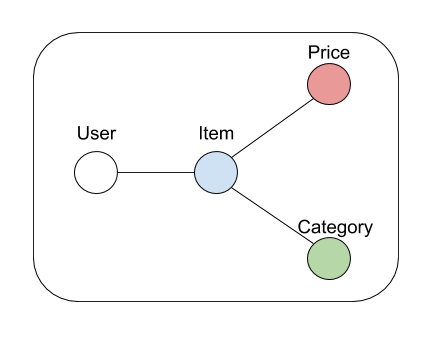
\includegraphics[scale=0.5]{figures/uipc.png}
    \caption{Illustration of the nodes in the simple extension of LightGCN.}
    \label{fig:uipc}
\end{figure}
We try to extend the implementation of LightGCN by changing the input parameters, where we construct the adjacency matrix containing the users, item, category and price graph, which is illustrated in \autoref{fig:uipc}.
The intuition behind the idea, is that the graph convolutions will capture the values of categories and price, so even if we do not use the embeddings for price and category, they will still influence users and items.
Let the user-item, item-price and item-category interactions matrix be $R \in \mathbb{R}^{I \times U + C + P}$, where $I$ denotes the number of items, $U, C, P$ denotes the number of users, categories and prices.
Each entry of $R_{ui}$ is 1 if user $u$ has rated item $i$. Otherwise it is 0.
If there is a connection in $R_{ic}$ or $R_{ip}$ this value is a hyperparameter $X$ with a value $x>0$, otherwise it is 0.
The adjacency matrix is obtained as follows:
\begin{gather}
    A =
    \begin{bmatrix}
        0   & R \\
        R^T & 0
    \end{bmatrix}
\end{gather}
The embeddings for users and price are calculated as follows,
\begin{equation}
    E^{(k+1)} = (D^{\frac{1}{2}}AD^{\frac{1}{2}}E^{(k)}),
\end{equation}
where $A$ is the adjacency matrix containing users, items, categories and price, and $D$ is a $(I + U + C + P)$ diagonal matrix, where $D_{ii}$ denotes the sum of the $i-th$ row in the adjacency matrix $A$.
The $0th$ layer embedding $E^{(0)} \in R^{(I + U + C + P)\times T}$, where $T$ is the embedding size.
We do not change anything else in LightGCN in this method.

